\chapter{Introduction\label{cha:chapter1}}

With the rising of the semantic web, the need for a standard for describing resources on the web has become more and more important. 
The Resource Description Framework (RDF) extends the Web’s linking structure by using URIs to name the relationships between resources and the two ends of the link. 
Different kind of scientist and engineers have been working with RDF:

\begin{itemize}
  \item \textbf{Data Scientists}:
  \begin{itemize}
      \item RDF aligns with their work on structured data, semantic queries, and knowledge graphs.
      \item They use RDF to model relationships, extract insights from interconnected datasets, and support machine learning on graph data.
  \end{itemize}
  
  \item \textbf{Computer Scientists and Engineers}:
  \begin{itemize}
      \item They focus on RDF’s theoretical foundations, optimization of storage and querying, and application development for the Semantic Web.
      \item They are often involved in creating RDF tools like RDF stores and query languages.
  \end{itemize}
  
  \item \textbf{Knowledge Engineers}:
  \begin{itemize}
      \item Specialize in designing ontologies and frameworks using RDF to represent knowledge in areas like AI, natural language processing, and expert systems.
  \end{itemize}
\end{itemize}

Despite all its capabilities, two main challenges must be faced when we work with RDF: Instance Generation and Data Visualization.
\\
\\
The instance generation process for A-Boxes resources is a complex and time-consuming task that requires a deep understanding of the underlying RDF schema and the relationships between resources. 
Creating few test instances for a small dataset is not an issue for a human, my with really large datasets, time starts playing its role.
\\
\\
Concerning Data Visualization are many grate tools on the web and application that support data visualization for RDF graphs.
Protégé is software that can be used to build both simple and complex ontology-based applications and allows to visualise many kind of schema structures \cite{protege}.
\\
\\
Several web-based tools and services are available for graph visualization, such as isSemantic \cite{} and RDF Grapher \cite{}.
These services provide an efficient and intuitive approach for visualizing RDF graph data, enabling users to assess the structural correctness of their graphs and verify the validity of relationships between nodes.
\\
Regardless of their extensive feature set, these services often struggle to find their place in an RDF developer’s workflow due to their lack of integration with commonly used IDEs and development toolchains.
\section{Motivation\label{sec:moti}}


This motivated me towards ...

\section{Theses and Scientific Contribution  \label{sec:objective}}

Objective - What kind of problem do you adress? Which issues do you try to solve? What solution do you propose? What is your goal?
'This thesis describes an approach to combining X and Y... The aim of this work is to...'

\section{Positioning within the Scientific Context \label{sec:scope}}

Scope - Here you should describe what you will do and also what you will not do. Explain a little more specific than in the objective section. 'I will implement X on the platforms Y and Z based on technology A and B.'

Conclude this subsection with an image describing 'the big picture'. How does your solution fit into a larger environment? You may also add another image with the overall structure of your component.

'Figure \ref{fig:intro} shows Component X as part of ...' 
\\
\begin{figure}[htb]
  \centering
  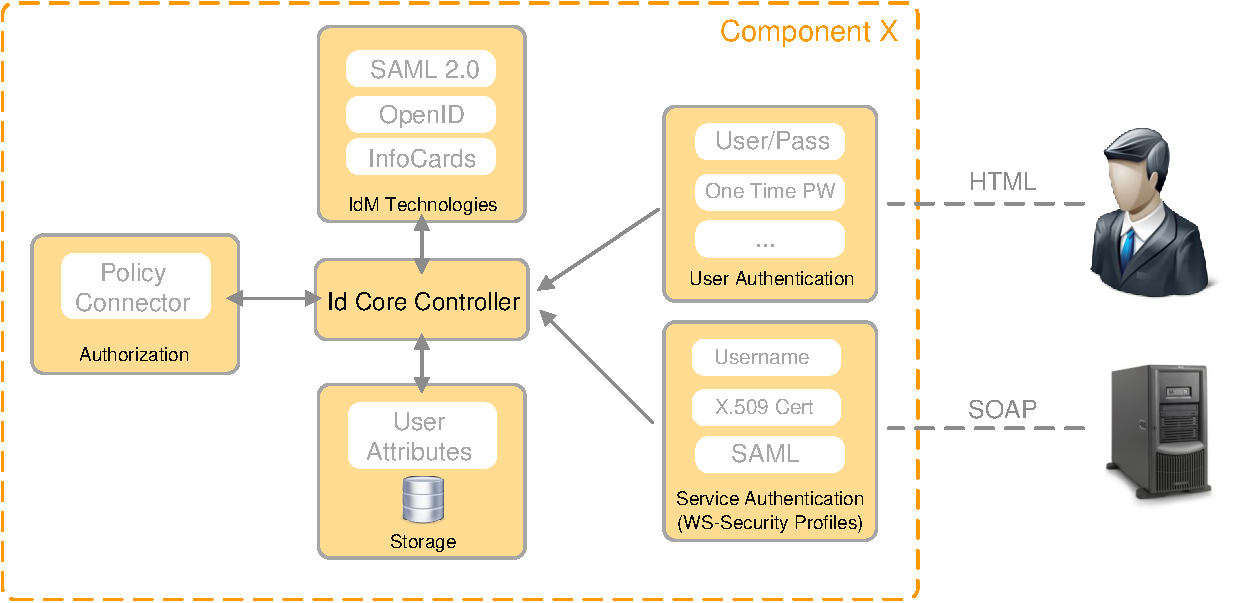
\includegraphics[width=9cm]{intro_example.pdf}\\
  \caption{Component X}\label{fig:intro}
\end{figure}

\section{Structure of the Work (and Methodology) \label{sec:outline}}

The 'structure' or 'outline' section gives a brief introduction into the main chapters of your work. Write 2-5 lines about each chapter. Usually diploma thesis are separated into 6-8 main chapters. 
\\
\\
\noindent This example thesis is separated into 7 chapters.
\\
\\
\textbf{Chapter \ref{cha:chapter2}} is usually termed 'Related Work', 'State of the Art' or 'Fundamentals'. Here you will describe relevant technologies and standards related to your topic. What did other scientists propose regarding your topic? This chapter makes about 20-30 percent of the complete thesis.
\\
\\
\textbf{Chapter \ref{cha:chapter3}} analyzes the requirements for your component. This chapter will have 5-10 pages.
\\
\\
\textbf{Chapter \ref{cha:chapter4}} is usually termed 'Concept', 'Design' or 'Model'. Here you describe your approach, give a high-level description to the architectural structure and to the single components that your solution consists of. Use structured images and UML diagrams for explanation. This chapter will have a volume of 20-30 percent of your thesis.
\\
\\
\textbf{Chapter \ref{cha:chapter5}} describes the implementation part of your work. Don't explain every code detail but emphasize important aspects of your implementation. This chapter will have a volume of 15-20 percent of your thesis.
\\
\\
\textbf{Chapter \ref{cha:chapter6}} is usually termed 'Evaluation' or 'Validation'. How did you test it? In which environment? How does it scale? Measurements, tests, screenshots. This chapter will have a volume of 10-15 percent of your thesis.
\\
\\
\textbf{Chapter \ref{cha:chapter7}} summarizes the thesis, describes the problems that occurred and gives an outlook about future work. Should have about 4-6 pages.